%# -*- coding: utf-8-unix -*-
%%==================================================
%% chapter01.tex for SJTU Master Thesis
%%==================================================

%\bibliographystyle{sjtu2}%[此处用于每章都生产参考文献]

\chapter{面向ASR的结构化单向辅助信息Multi-view语言模型}
\label{chap:struclm}



%%%%%%%%%%%%%%%%%%%%%%%%%%%%%%%%%%%%%%%%%%%%%%%%%%%%%%%%%%%%%%%%%%%%%%

\section{现有结构化语言模型研究及现状} 
\label{sec:struclm}

\ref{fig:LSTM} 展示了三种基础的在LSTM语言模型上的扩展结构,这三种结构正在被广泛使用,也会作为本文工作的基础工作和实验基线。 
可以初步看出Multi-task、Multi-view和Joint train模型的结构特征和对比的区别。
Multi-task是有多个输出和训练准则,同样有多个训练标注。
Multi-view则是有多个输入,直观理解是训练一个目标模型,有多个辅助特征的输入。
而Joitn train则是前两者进行一定程度的结合,偶尔会有一些时序上的错位,比如上一个时刻的第二个任务的的输出作为当前时刻的输入等等。

模型细节和优劣将在后文分别进行描述,实验结果和比较,以及分析将会在第五章呈现。
如上文介绍所说,为了进一步提升语言模型的性能,研究者们在语言模型的结构化研究中做了很多工作。其中就有在训练模型的过程中加入额外信息的多视角学习,通过加入词层面的辅助信息和当前词一起训练以提升语言模型的性能\cite{shi2012towards}. 
额外的辅助信息包括词性标注(part of speech,POS),命名实体识别(named entity recognition,NER),语法块( chunking)\cite{Tjong2000Introduction},句子的环境信息,语法解析信息等。
这些辅助信息被合并到Multi-view模型中,甚至可以作为联合模型逐帧一起训练\cite{shi2015integrating}.但是虽然这些工作在混淆度的指标上有非常大的提升,但是在语音识别方向的重打分任务的词错误率(WER)和句子错误率(SER)中却依然没有提升,甚至有的还有所下降\cite{shi2012towards}\cite{shi2015integrating}。



\subsection{multi-task语言模型}

随着LSTM RNN模型被证实是一效果很好的模型,很多的研究工作便在此模型的基础上展开,语言模型也不例外。
为了获得更进一步的提升,更多有效的复杂的网络结构也应运而生,比如说本章要讨论的结构化语言模型的研究。


 \begin{figure}[tbhp!]
    \small
    \centering
    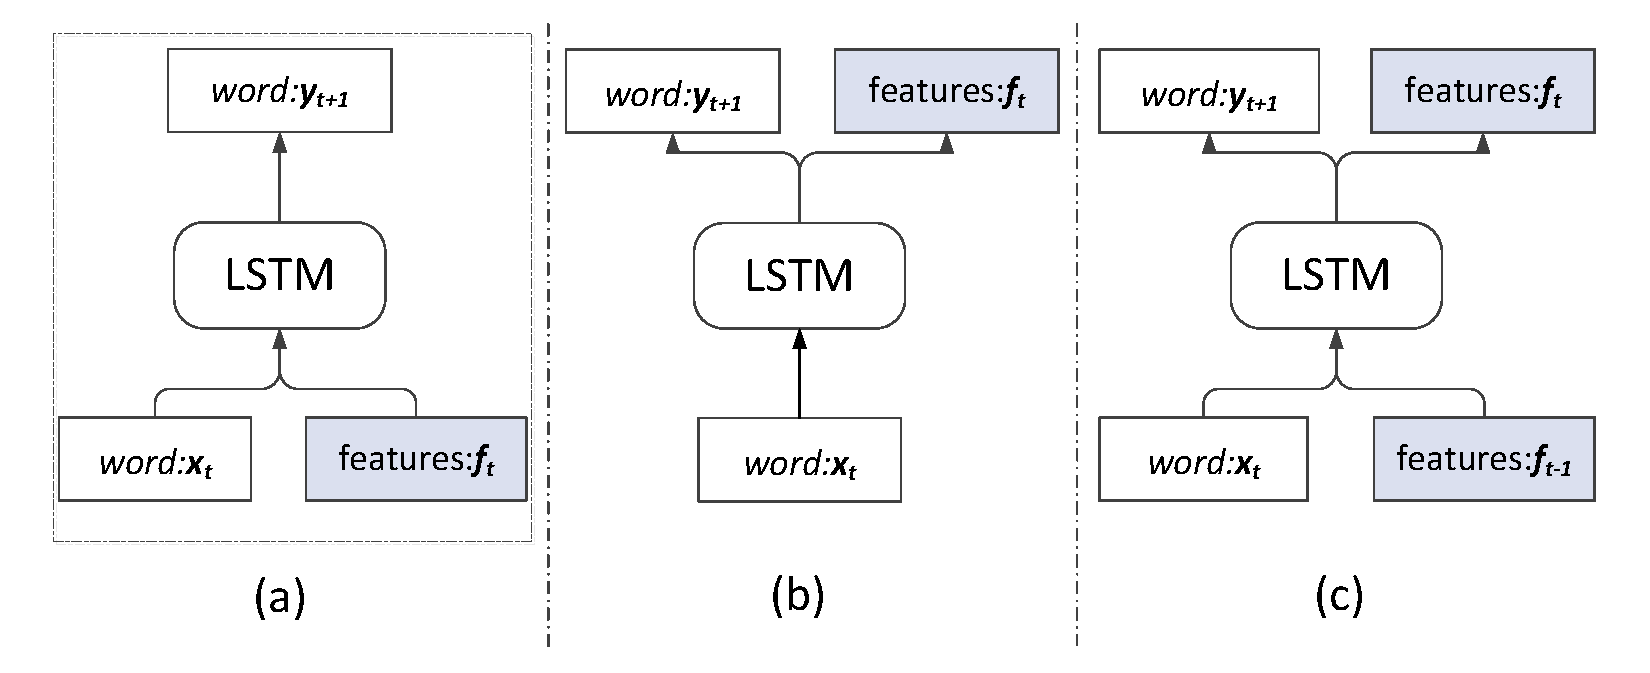
\includegraphics[width=\linewidth]{struclm/LSTM.pdf}
    \caption{{\it (a)Multi-view LSTM语言模型. (b)Multi-task LSTM语言模型. (c)Joint train LSTM语言模型.}}
    \label{fig:LSTM}
  \end{figure}
\subsection{Multi-task语言模型}
正如图\ref{fig:LSTM}$(b)$所展示的, 在Multi-task模型结构中,语言模型被设计成和其它的模型一起训练。
它们共享输入和一部分的隐层\cite{Collobert2008A}, 

However most researches on multi-task structure show that usually performance gain is achieved in the cooperating task, instead of LM task itself.


\subsection{multi-task模型结构}
\subsection{multi-task语言模型的表现}

\subsection{Multi-view语言模型}
Considering that some extra linguistic features might contribute to  language modeling, word and sentence level features were introduced in LM \cite{shi2012towards}. This model have multi inputs, which contains different views of information. So it is called multi-view model (see \ref{fig:LSTM}$(a)$).

As argued in Section 1, research on this kind of model shows improvements on perplexity and word prediction accuracy (WPA), but integrating this model with ASR did not lead to commensurate improvements \cite{shi2015integrating}.
That is to say, the straightforward combination of words and features as the inputs of a language model do not contribute to speech recognition.

Our proposed model is based on the multi-view structure, but is specially tailored for ASR task by using word-synchronized auxiliary feature.

\subsubsection{multi-view语言模型的结构}
\subsubsection{multi-view的多视角特征信息介绍}
\subsubsection{multi-view语言模的表现}

\subsection{Joint-train语言模型}
Other works combined the multi-task structure with multi-view structure, which is shown in Figure~\ref{fig:LSTM}$(c)$. Not only multiple tasks were trained together, but also the inputs of this model were multi-view. LM was jointed with other spoken language understanding (SLU) or natural language process (NLP) task, some models of improved version are researched. Better than multi-task models, these works show slight improvement in PPL and ASR-rescoring, but more promotion is gained in the cooperating task \cite{Liu2016Joint}.


\subsubsection{Joint-train语言模型结构}
\subsection{研究动机和思路}
我们猜测造成上述现象的主要原因是因为那些额外的辅助信息用的都是标准的标注算法,比如最大熵算法和双向LSTM模型,这些模型虽然表现优秀,但是在标注过程中用到了全局信息。
也就是不仅用到了前文的信息,更用到了后文的信息。
这就意味着在训练语言模型的时候,给当前词的辅助信息中包含后文信息,然后语言模型再用后文信息去预测后面的词。有点类似于信息作弊的感觉。这也是为什么在PPL任务上表现优秀的原因。

那为什么又在重打分任务中没有提升呢,这可能是因为重打分任务中的n-best集合(在第四章实验部分详细介绍)中的各种句子是本身就不合理的(语言模型得分很低),用不合理的后文信息得到的标注也会存在问题。
也就是意味着用不合理的后文信息预测后面的词,自然会出现偏差。

为了验证和解决这个问题,为了使得结构化语言模型不仅提升了语言模型的某个指标(PPL),更是要使得它在实际应用中(ASR任务)中有所提升,我们提出仅仅使用单向的辅助信息去训练结构化的语言模型。

基于这个思想,我们进行了一系列研究工作。
在我们的工作中,我们使用一个单向LSTM标注模型去进行双向信息的单向化。保证从词模型中出来的标注信息仅仅会包含历史信息,而不包含未来信息。
紧接着,标注模型的输入被作为Multi-view语言模型的一个输入接入到一个LSTM语言模型结构中。
在这种模型结构下,存在不同的训练方法,我们总共尝试了五种不同的训练方法。
最后我们将我们提出的模型和前人的相似结构模型进行多方位的在PPL和ASR任务上的比较。
%%%%%%%%%%%%%%%%%%%%%%%%%%%%%%%%%%%%%%%%%%%%%%%%%%%%%%%%%%%%%%%%%%%%%

\section{单向辅助信息模型的辅助信息选取}
\subsection{词性标注} 
词性是用来表示一个词的性质的,例如名词、形容词、动词等,每个词都有词性,有的甚至不止一种词性,根据在句子中所扮演的成分不同而有区别。

词性标注(Part-Of-Speech Tagger,POS Tagger)为以前无限的语言模型提供了有限的句法信息,例如限定词往往紧随其后的是名词。此外,对语言模型添加词性标记可以被看作是一种平滑,对于那种在训练数据中出现概率很小的单词,加入词性的语言模型相当于给他们分配了更一般的抽象类,从而增大他们的概率使其不再接近于0,从而可以更好的处理它们[20]。
词性标注是自然语言处理(NLP,Natural Language Processing)的范畴,

词性标注任务研究如何判别一个句子中的每个词的词性类别,如名词、动词、形容词等。
词性是最基础也最常用的一类特征。
在大量涉及自然语言的应用,如语音合成、句法分析、机器翻译中,词性都是必不可少的输入特征,其识别结果的正确性对这些系统的最终表现也有着显著的影响。
词性标注是一个典型的标注任务,它的输入为一串词序列,每个词所对应的词性即为输出,如图\ref{fig:possample}所示,


 \begin{figure}[tbhp!]
    \small
    \centering
    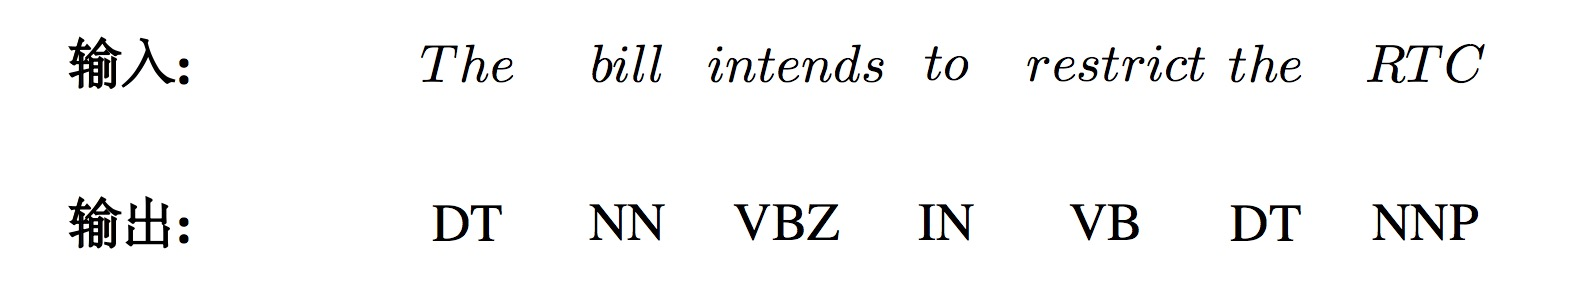
\includegraphics[width=\linewidth]{struclm/possam.jpeg}
    %\caption{{\it (a)Multi-view LSTM语言模型. (b)Multi-task LSTM语言模型. (c)Joint train LSTM语言模型.}}
    \caption[词性标注任务输入输出示例]{\textbf{词性标注任务输入输出示例。}输入为词序列(即句子),输出为该句子的词性标注序列。}
    \label{fig:fpossample}
  \end{figure}

本文采用的词性标注工具是斯坦福大学的开源词性标注工具,具有各种语言之分。输入到词性标注工具中的文本是已经经过分词处理的中文文本,若是英文文本可以直接进行词性标记,没有分词这个步骤。每个词的词性并不是固定的,例如“游泳”既可以是动词,也可以是名词,具体标记的算法由词性标记工具实现。

获得词性标注之后,我们用处理词向量的方式来处理词性标注。同样我们建立一个词性的词表,对于每一个词性,将其映射到词表上,对应的位置为$1$,其它为$0$,最后得到的就是一个一维的长度为词性的个数,对应位置为$1$其它为$0$的向量,如公式

\begin{equation}
    {pos_t}(i)=\left\{  
             \begin{array}{lr}  
             1  ({wp_t} = {vp_i}) \\
             0  ({wp_t} \not= {vp_i}) 
             \end{array}  
	\right.  
\end{equation}

其中${pos_t}$ 为当前$t$时刻的单词对应的词性所表示的向量,$i$表示向量的第$i$维, ${wp_t}$表示当前的单词所对应的词性, ${vp_i}$表示词性的词表中第$i$个词性。它即是词性的特征向量。

\subsection{命名实体识别} 
命名实体识别(Named Entity Recognition,简称NER),又称作“专名识别”,是指识别文本中具有特定意义的实体,主要包括人名、地名、机构名、专有名词等。
命名实体识别也是信息抽取(Information Extraction)相关任务的核心技术,因此有着很高的研究价值。
通常包括两部分:(1)实体边界识别;(2) 确定实体类别(人名、地名、机构名或其他)。英语中的命名实体具有比较明显的形式标志(即实体中的每个词的第一个字母要大写),所以实体边界识别相对容易,任务的重点是确定实体的类别。和英语相比,汉语命名实体识别任务更加复杂,而且相对于实体类别标注子任务,实体边界的识别更加困难。


与语块切分类似,命名实体识别也是一个切分任务,同样可以使用IOBES的标注策略转化为标准标注任务,输入输出样例如图\ref{fig:nersample}所示。

\begin{figure}[tbhp!]
\small
\centering
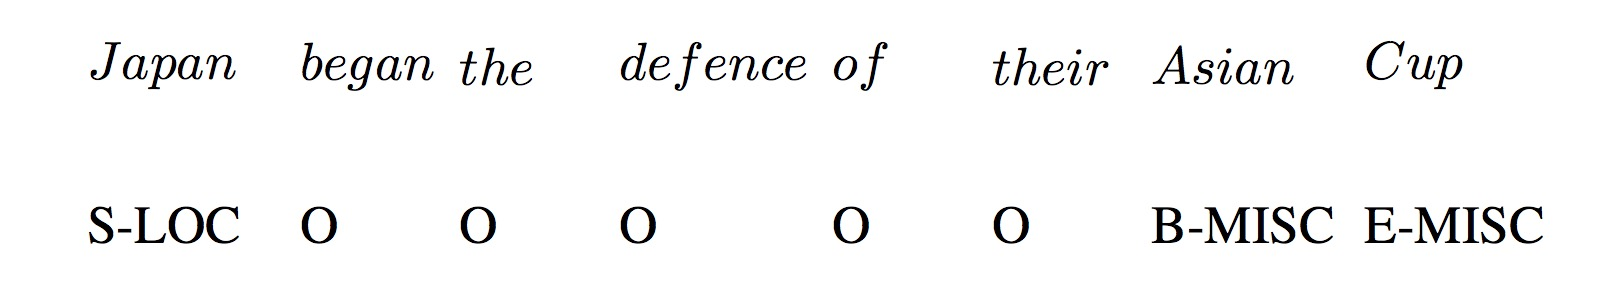
\includegraphics[width=\linewidth]{struclm/nersam.jpeg}
%\input{struclm/graph.nersample.tex}
\caption[命名实体识别任务输入输出示例]{\textbf{命名实体识别任务输入输出示例。}输入为词序列,输出为该句子的命名实体识别标签序列(使用了IOBES标注策略)。}\label{fig:nersample}
\end{figure}



\subsection{语法块标注} 
语块切分任务也称为浅层句法分析(shallow parsing),它研究如何把句子切分成不同的句法模块,如名词词组(Noun Phrase,NP)、动词词组(Verb Phrase,VP)、介词词组(Preposition Phrase,PP)等。
与词性标注类似,语块切分同样也是一种常用且重要的特征,对于句法分析、语义理解任务尤其重要。
与词性标注不同,语块切分是一个分割(segmentation)任务。
分割任务需要明确指定当前词所属类别的边界,边界内的词都属于同一类别,简单套用本章开头定义的标注模型不能确保上述限制条件。
不过通过使用特定的标注策略如IOBES、IOB、IOE等,语块切分任务也可以转成一个标准的标注任务。

以IOBES标注策略为例,该标注策略将每个原有的类别X扩展成四个子类别B-X,I-X,E-X与S-X,每个子类分别表示当前词属于$X$类且处于分割的开始位置(\textbf{B}egin),中间位置(\textbf{I}ntermediate),结尾(\textbf{E}nd)与单词分割(\textbf{S}ingle)。
此外,该策略还额外引入标签$O$表示该标签不属于任何分割(\textbf{O}ther)。
使用该标注策略的语块切分系统,首先预测每个词的IOBES扩展后的子类别,然后以$B$,$E$,$S$,$O$为边界将输出切分成段。
使用IOBES策略的输出与切分结果示例如图\ref{fig.tagschemesample}所示。
\begin{figure}[tbhp!]
\small
\centering
%\input{struclm/graph.chunksam1.jpeg}
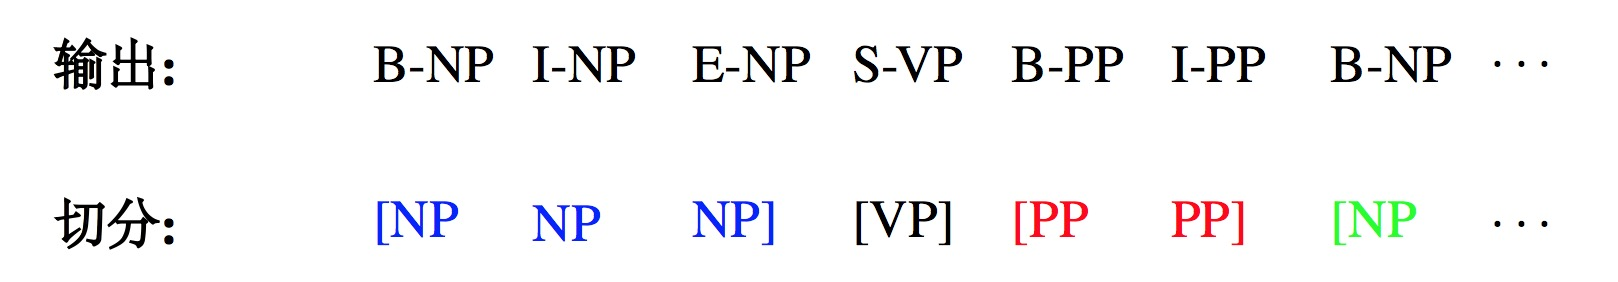
\includegraphics[width=\linewidth]{struclm/chunksam1.jpeg}
\caption[IOBES标注策略输出与切分示例]{\textbf{IOBES标注策略输出与切分示例。}}\label{fig.tagschemesample}
\end{figure}

IOB,IOE与IOBES类似,只是更加简化只有三个子类。
表\ref{table.tagscheme}展示比较了上述三类标注策略。
\begin{table}
\centering
\begin{tabular}{|c|c|c|c|c|c|}
\hline
Scheme & Begin & Inside & End & Single & Other \\
\hline
IOB & B-X & I-X & I-X & B-X & O \\
\hline
IOE & I-X & I-X & E-X & E-X & O \\
\hline
IOBES & B-X & I-X & E-X & S-X & O \\
\hline
\end{tabular}
\caption[IOB,IOE,IOBES标注策略比较]{\textbf{IOB,IOE,IOBES标注策略比较。}}\label{table.tagscheme}
\end{table}
在实际应用中,这三种标注方式都有工作使用,关于他们的优劣目前也无定论。
本文选择使用IOBES策略。
关于语块切分的输入输出样例如图\ref{fig.chunksample}所示。
\begin{figure}[tbhp!]
\small
\centering
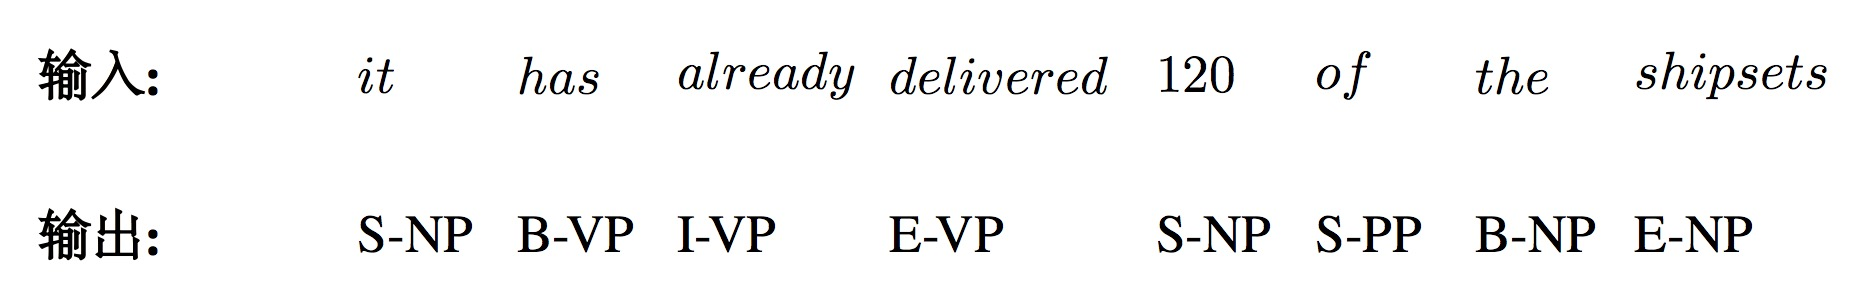
\includegraphics[width=\linewidth]{struclm/chunksam2.jpeg}
%\input{struclm/chunksam2.jpeg}
\caption[语块切分任务输入输出示例]{\textbf{语块切分任务输入输出示例。}输入为词序列,输出为该句子的语块切分标签序列(使用了IOBES标注策略)。}\label{fig.chunksample}
\end{figure}



\section{单向辅助信息的Multi-view语言模型结构}
\label{Multi-view}
我们的模型总共由两个部分组成:第一部分是用来生成单向辅助信息特征的标注模型;另一个是一个和标注模型链接在一起的Multi-view语言模型。
对于这两个模型,我们都是用的单层单向LSTM模型,并且将这两个模型以此层面的粒度链接在一起。关于模型的详细介绍和数学基础将在下文给出。


\subsection{单向LSTM标注模型部分}
\label{sec:psd-ac-conf}
标注模型是一种分类模型,一个标注模型是通过训练得到为每个输入序列找到它所属类别并输出。
神经网络现在被广泛用于各种标注模型中\cite{schmid1994part},因为它能大幅图提升传统统计学标注模型的性能。
其中双向神经网络更为普遍\cite{Wang2015A},由于前后文信息的紧密结合,更是使得标注模型进一步提升。
神经网络的标注模型是根据输入输出它所属的类别的概率分布。



  \begin{figure}[tbhp!]
    \small
    \centering
    %\tikzset{
label/.style={
  rectangle,
  draw=none,
  text centered,
  inner sep=0.6em,
},
namelabel/.style={
  rectangle,
  draw=none,
  text width=12em,
  inner sep=0.6em,
  align=left
},
bigcircle/.style={
  rectangle,
  rounded corners,
  draw,
  minimum width=3em,
  text centered,
  inner sep=0.3em,
}
}

\scriptsize
\begin{tikzpicture}[x=1em, y=1em, >=stealth]
%nodes
\node[bigcircle](fht1) at (-5.5,0){LSTM};
\node[bigcircle](fht2) at (0,0){LSTM};
\node[bigcircle](fht3) at (5.5,0){LSTM};

\node[label](x0) at (-9,-4){$\dots$};
\node[label](x1) at (-5.5,-4){\underline{$w_{t-1}$}};
\node[label](x2) at (0,-4){\underline{$w_{t}$}};
\node[label](x3) at (5.5,-4){\underline{$w_{t+1}$}};
\node[label](x4) at (9,-4){$\dots$};

\node[label](y0) at (-9,4){$\dots$};
\node[label](y1) at (-5.5,4){\underline{$f_{t-1}$}};
\node[label](y2) at (0,4){\underline{$f_{t}$}};
\node[label](y3) at (5.5,4){\underline{$f_{t+1}$}};
\node[label](y4) at (9,4){$\dots$};

\node[namelabel](textoutputs) at (-14,4){Outputs:};
\node[namelabel](textbklayer) at (-14,0){Hidden Layer(LSTM):};
\node[namelabel](textinputs) at (-14,-4){Inputs:};

\draw[->](fht1) to (y1);
\draw[->](fht2) to (y2);
\draw[->](fht3) to (y3);

\draw[->] (-10,0) -- (fht1);
\draw[->](fht1) -- (fht2);
\draw[->](fht2) -- (fht3);
\draw[->](fht3) -- (10,0);

\draw[->] (x1) -- (fht1);
\draw[->] (x2) -- (fht2);
\draw[->] (x3) -- (fht3);


\end{tikzpicture}

    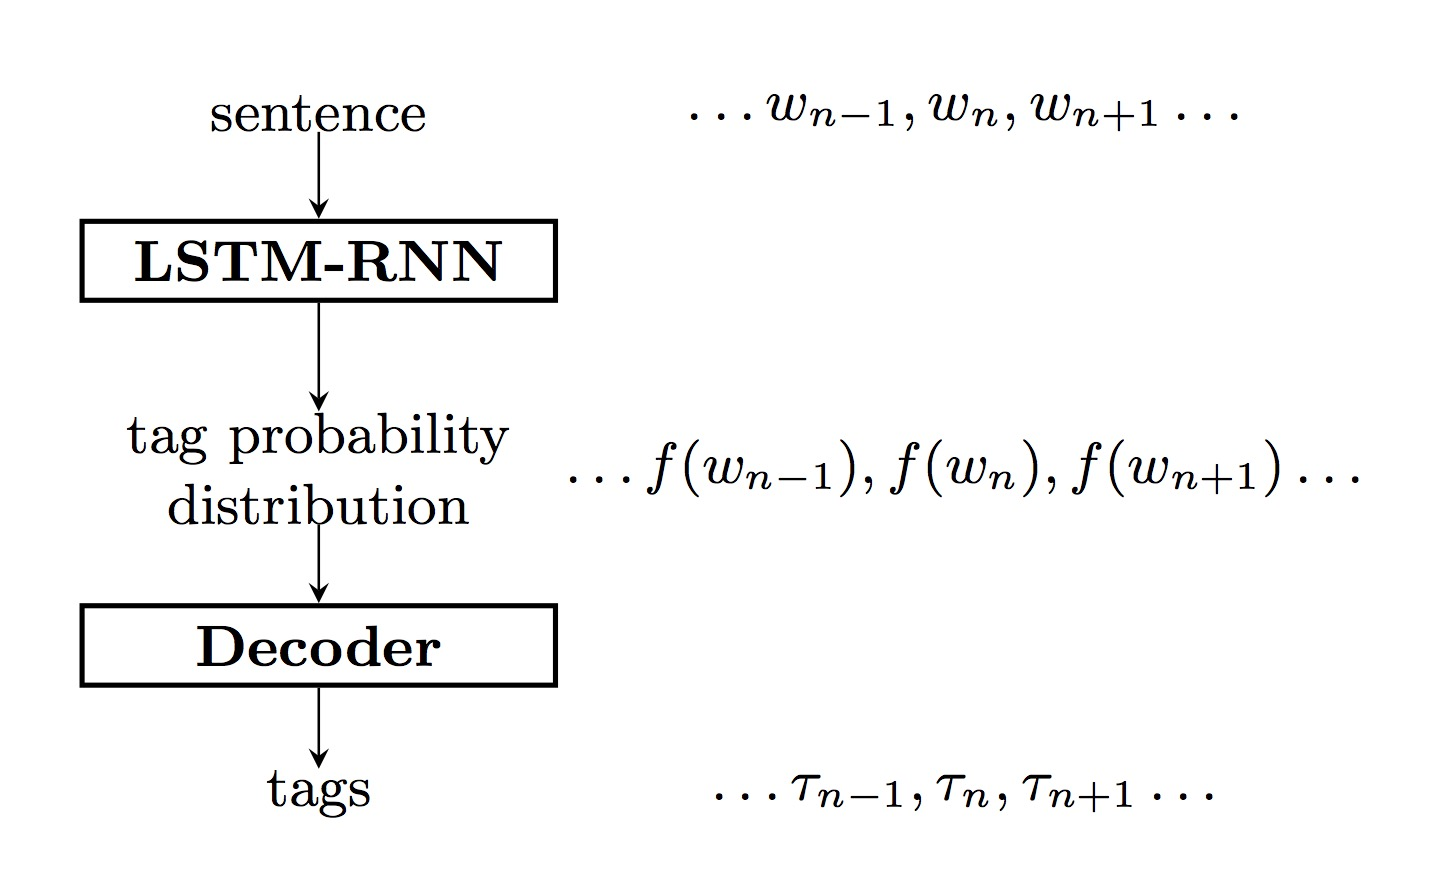
\includegraphics[width=\linewidth]{struclm/tagging.jpeg}
    \caption{{\it uni-directional LSTM tagging model}}
    \label{fig:tagging}
  \end{figure}

不过如前文所说,本文这里必须使用单向神经网络。
另外在我们的验证实验和我们的三种标注任务中,双向LSTM模型相比于相同参数的单向LSTM模型仅仅有非常微小的性能提升。
如图\ref{fig:tagging}所示,这是一个单向模型的模型结构示意图,
一个LSTM网络结构就和RNN一样有隐层的递归的自环,其中每个隐层单元被替换成了具有长短时记忆功能的LSTM单元。
在后文中,LSTM记忆单元被统一表示成$\mathcal{L}$。另外为了避免混淆,标注模型和语言模型的LSTM记忆单元分别被表示成 $\mathcal{L}_{\tt{tag}}$和$\mathcal{L}_{\tt{LM}}$。



向量$\bm{w}_t$使用one hot编码来表示当前时刻$t$的当前词,这个one hot向量也同时是$\mathcal{L}_{\tt{tag}}$和$\mathcal{L}_{\tt{LM}}$.

接下来,这个词的此嵌套$\bm{x}_t$可以这样得到:
	\begin{equation}
    \bm{x}_t = E_{tag}\bm{w}_t
	\end{equation}
这里$E_{tag}$ 是指标注模型的词嵌套矩阵。    

单向LSTM标注模型的输出层 $\bm{h}_t$ 由下述公式计算得到:  
	\begin{equation}
    \bm{h}_t = \mathcal{L}_{\tt{tag}}(\bm{x}_t,\bm{h}_{t-1})
	\end{equation}
其中LSTM计算单元$\mathcal{L}$内部的详细的函数表达式如公式ref{eq:memoryb}所展示的这样:

其中 $\sigma$ 是逻辑函数 (sigmoid), 以及$i$, $f$, $o$ and $c$ 分别表示 \textit{input gate}、 \textit{forget gate}、 \textit{output gate} and \textit{cell} 激励向量.



$\bm{f}_t$ 是标注模型的输出,这是个总和为$1$的向量,表示输出的标注分类的概率分布, 同样的它可以根据模型的隐层LSTM记忆单元求得,公式如下:
	\begin{equation}
    \bm{f}_t = softmax(W_{ho}\bm{h}_{t}+\bm{b}_y)
	\end{equation}	
其中softmax是归一化函数,目的是让概率分布总和为1.




 %and vector $\mathbf{s}(t-1)$ represents the hidden layer output in the previous time step.
根据截止到目前所描述的LSTM-RNN语言模型,观测到的每个时刻的模型的输出概率分布和其它时刻是相互独立的,仅仅根据数据训练得出。
然而,在有些任务中,比如说NER和Chunking任务中,标注之间具有一些隐含的规则,它们之间和前后的标注具有强关联性。其中一部分种类仅仅能存在在部分特定的种类之后,而一部分不能存在于某些之后。比如说NN-B(名字块开头)后面不可能跟VV-E(动词块)结尾,加了类似于这些规则之后标注模型的准确率会有一定的提升。


为了将上述的标注之间的约束关系利用起来,
我们在每一步中引入转化矩阵的概念,如果两个标注类别之间可以连接,则矩阵为1,否则为0。矩阵是单向的,比如B能在A后面出现,则$matrix[A][B]=0$,而B不一定能在A之前出现,若不能则$matrix[B][A]=0$。
这个矩阵和标注模型的概率分布一起进行解码\cite{Wang2015A},便能得到概率最大的标注序列。 
这个解码过程可以用经典的Viterbi算法\cite{Andrew1967Viterbi}完成。

在本文中,解码过程被表示成$\mathcal{D}(\cdot)$,
解码过程的输出$\mathbf{\tau}_t$ 是一系列最终预测得到的标注序列,它们同样用one hot向量表示如下:

	\begin{equation}
    \bm{\tau}_t = \mathcal{D}(\bm{f}_t)
	\end{equation}

到此我们可以发现,标注模型的输出传到语言模型中可以有两种表示:第一种是概率分布的序列,第二种是经过Viterbi解码后得到的确切的one hot序列。



\subsection{Multi-view语言模型部分}
\label{sec:psd-ac-conf}
图\ref{fig:selfpos} 展现了我们的仅用前文辅助信息的Multi-view LSTM语言模型架构。

  \begin{figure}[tbhp!]
    \small
    \centering
    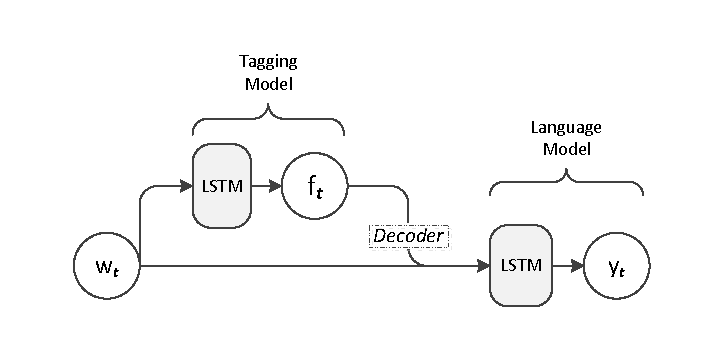
\includegraphics[width=\linewidth]{struclm/selfpos.pdf}
    \caption{{\it multi-view LSTM  language model with word-synchronized auxiliary feature}}
    \label{fig:selfpos}
  \end{figure}


我们提出的模型是一个和单向标注模型连接起来的Multi-view语言模型。

语言模型的第一个输入 $\bm{w}_t$ 是一个代表当前词的one hot向量 , 这个向量同时也是标注模型的输入。
第二个输入是标注模型部分的输出,可以是经过Viterbi解码之后的ont序列,也可以是直接的概率分布。
无论这个解码过程有没有进行,我都对于两者都在第四章的实验部分进行了实验与比较。
它们的不同点也体现在输入部分的公式上,
如果使用了Viterbi解码,语言模型的第二个输入将会是:
	\begin{equation}
\bm{\zeta}_t=W_{tag}\bm{\tau}_t + E_{word}\bm{w}_t 
	\end{equation}
其中$\bm{\tau}_t$ 是解码部分输出的one hot向量。
否则,语言模型的输入是:
	\begin{equation}
\bm{\zeta}_t=W_{tag}\bm{f}_t +  E_{word}\bm{w}_t 
	\end{equation} 
其中$\bm{f}_t$ 是标注模型的概率分布形式的输出。
$E_{word}$ is 是词嵌套矩阵,$W_{tag}$ 是标注模型到语言模型的隐层之间的参数矩阵。它们将会在每个时序点被加起来作为语言模型最终的输入。



%The same as tagging model, as $\bm{\sigma}_t$ is the input of $\mathcal{L}_{\tt{LM}}$.
LSTM语言模型的隐层的输出为 $\bm{h}_t$,它的计算公式是: 
	\begin{equation}
    \bm{h}_t = \mathcal{L}_{\tt{LM}}(\bm{\zeta}_t,\bm{h}_{t-1})
	\end{equation}
LSTM记忆快的具体函数 $\mathcal{L}$ 的公式已经在上一小节介绍过了。
$\bm{y}_{t}$ 是语言模型的输出,
表示预测的下一个词的概率分布$P(\bm{x}_{t+1}|\bm{x}_1\mathord{:}\bm{x}_t)$, 
它同样根据LSTM隐层单元得到,公式如下: 
	\begin{equation}
    \bm{y}_{t} = softmax(W_{ho}\bm{h}_{t}+\bm{b}_y)
	\end{equation}	
    
上述就我我们单向自信息Multi-view语言模型的结构描述。
    
\section{模型的训练方法}
我们提出的模型由两部分组成:标注模型和语言模型。
语言模型训练过程遵循标准约定,先计算每个单词的交叉熵,然后进行反向传播。
我们采用基于小批量的随机梯度下降法(SGD)作为优化方法。
但是由于语言模型和标注模型的连接方式的不同,我们尝试了五种不同的训练方法,并进行实验和比较。
五种训练方式如下:

1) 将LSTM标记模型作为一个独立的模型进行训练,在训练多视角语言模型时将标注模型固定,并不继续进行训练更新。五种方式中只有这种方法才能利用解码过程,因为后面的方法需要训练标注模型,但解码过程出来的结果是确定的值,无论是解码还是采样过后都不支持将误差从语言模型传递到标注模型,从而不支持继续训练标注模型。其优势在于,解码器有利于提升标注模型,但它的缺点是在语言模型训练时标注模型不能更新。

2)提前对LSTM标注模型进行训练,不同于第一种方法,这种方法中标注模型也会在训练语言模型的时候进行训练和更新,此时标注模型的输出是以概率分布的形式输入到语言模型中。标注模型的学习率下降速度和语言模型保持一致。这个方法有个致命缺点是:训练好的标注模型会因为不恰当的学习率在训练语言模型的时候训毁。

3)并不事先训练好标注模型,而是对其进行随机初始化,然后整个系统——标注模型和语言模型部分一起记性训练,使用相同的学习率。 


4)第三种和第四种方式都是实用的相同学习率,本方法在第二种训练方法的基础上,采用学习率稳定算子$\beta$自适应算法 \cite{Ghahremani2016Self}\cite{Liu2016investigation} 进行模型的更新,目的是为了合理的调整学习旅使得在不同的模型部分使用适合于它自己的学习率。比如第二种方法中标注模型是事先训练好的, 调整幅度就应该非常小。 

5)与第四种方式相似, 这个方法是在第三种方法的基础上加入稳定算子$\beta$自适应算法。

由于我们所提出的模型的最佳训练方法是未知的,所以这五种方法都在实验中进行了测试和评估。结果如第$4$章实验部分所示。






